
In this section we follow a prepared example that can be found in:
\begin{center}
{\color{blue}\url{https://github.com/drinkingkazu/Example}}
\end{center}
You might have already checked out this repository as this was mentioned briefly
in the introductory section (see Sec.\ref{sec:build}). 
If not, can certainly checkout under \UserDev:
\begin{lstlisting}
  > cd $LARLITE_USERDEVDIR
  > git clone https://github.com/drinkingkazu/Example
\end{lstlisting}

This repository contains following packages:
\begin{itemize}
\item {\ttfamily Empty} for the simplest example to introduce a simple \CPP class
\item {\ttfamily Function} for demonstrating a \CPP function to be exported into a dictionary
\item {\ttfamily Dependent} for showing how to make inter-package dependencies
\item {\ttfamily DataProduct} as an example of how to store a class instance into a file
\end{itemize}
where we skip the first item, {\ttfamily Empty}, as that has been covered in the previous section.

\subsection{\CPP Functions}
I would like to avoid a confusion: \CPP class is an extension of data structure. In particular,
you do not have to make \CPP class for inventing one or a few functions. Just like we have done
some practice with \CPP class, it would be useful to have \CPP functions in a dictionary.
The point of this package is to show how one can do this.

Take a look at {\ttfamily MyFunctions.h} and {\ttfamily MyFunctions.cxx} source code: there, I defined
functions:
\begin{lstlisting}
  void hello_world();
  Beer Brew(const int age);
\end{lstlisting}
where {\ttfamily example::Beer} is a \CPP class defined in {\ttfamily Beer.h}: it's very very simple class for
playing around unlike the sophisticated name.

Now a compilation works just as expected, and there is nothing special about these functions.
What you may find useful is a format to declare above functions in {\ttfamily LinkDef.h}:
\begin{lstlisting}
#pragma link C++ function  example::hello_world()+;
#pragma link C++ function  example::Brew(const int)+;
\end{lstlisting}
As you can see, a) you do not specify the return type of the function, and b) you only need to specify
the argument types. 

You can try executing an example script {\ttfamily mac/example.py} which calls those functions. 
Take a look at the script's contents and see if that makes sense (... and ask a question if you have any!).
{\color{red}\bf There is one caveat}, however: currently \ROOT seems to require \CPP class compiled
in the same library to be instantiated {\bf before} \CPP functions to be called. The author will
open a ticket for this to be fixed.

\subsection{\ROOT Data Product Class}
Once you get familiar with all LArLite features, you might want to store \CPP object in a file
as a {\ttfamily data product}. The easiest (and recommended) method is to use a \ROOT file.
A rule of the thumb is that any \CPP class that is generated with a \ROOT {\it dictionary} can
be stored in a \ROOT file. You can find details in the \ROOT manual.

If you use LArLite as your code development environment, \ROOT dictionary file is always
generated and built at compilation stage of your package. 

An example can be found in the package {\ttfamily DataProduct}.
There, a data product class called {\ttfamily example::Scotch} is defined. 

\begin{figure}[htb]\begin{center}
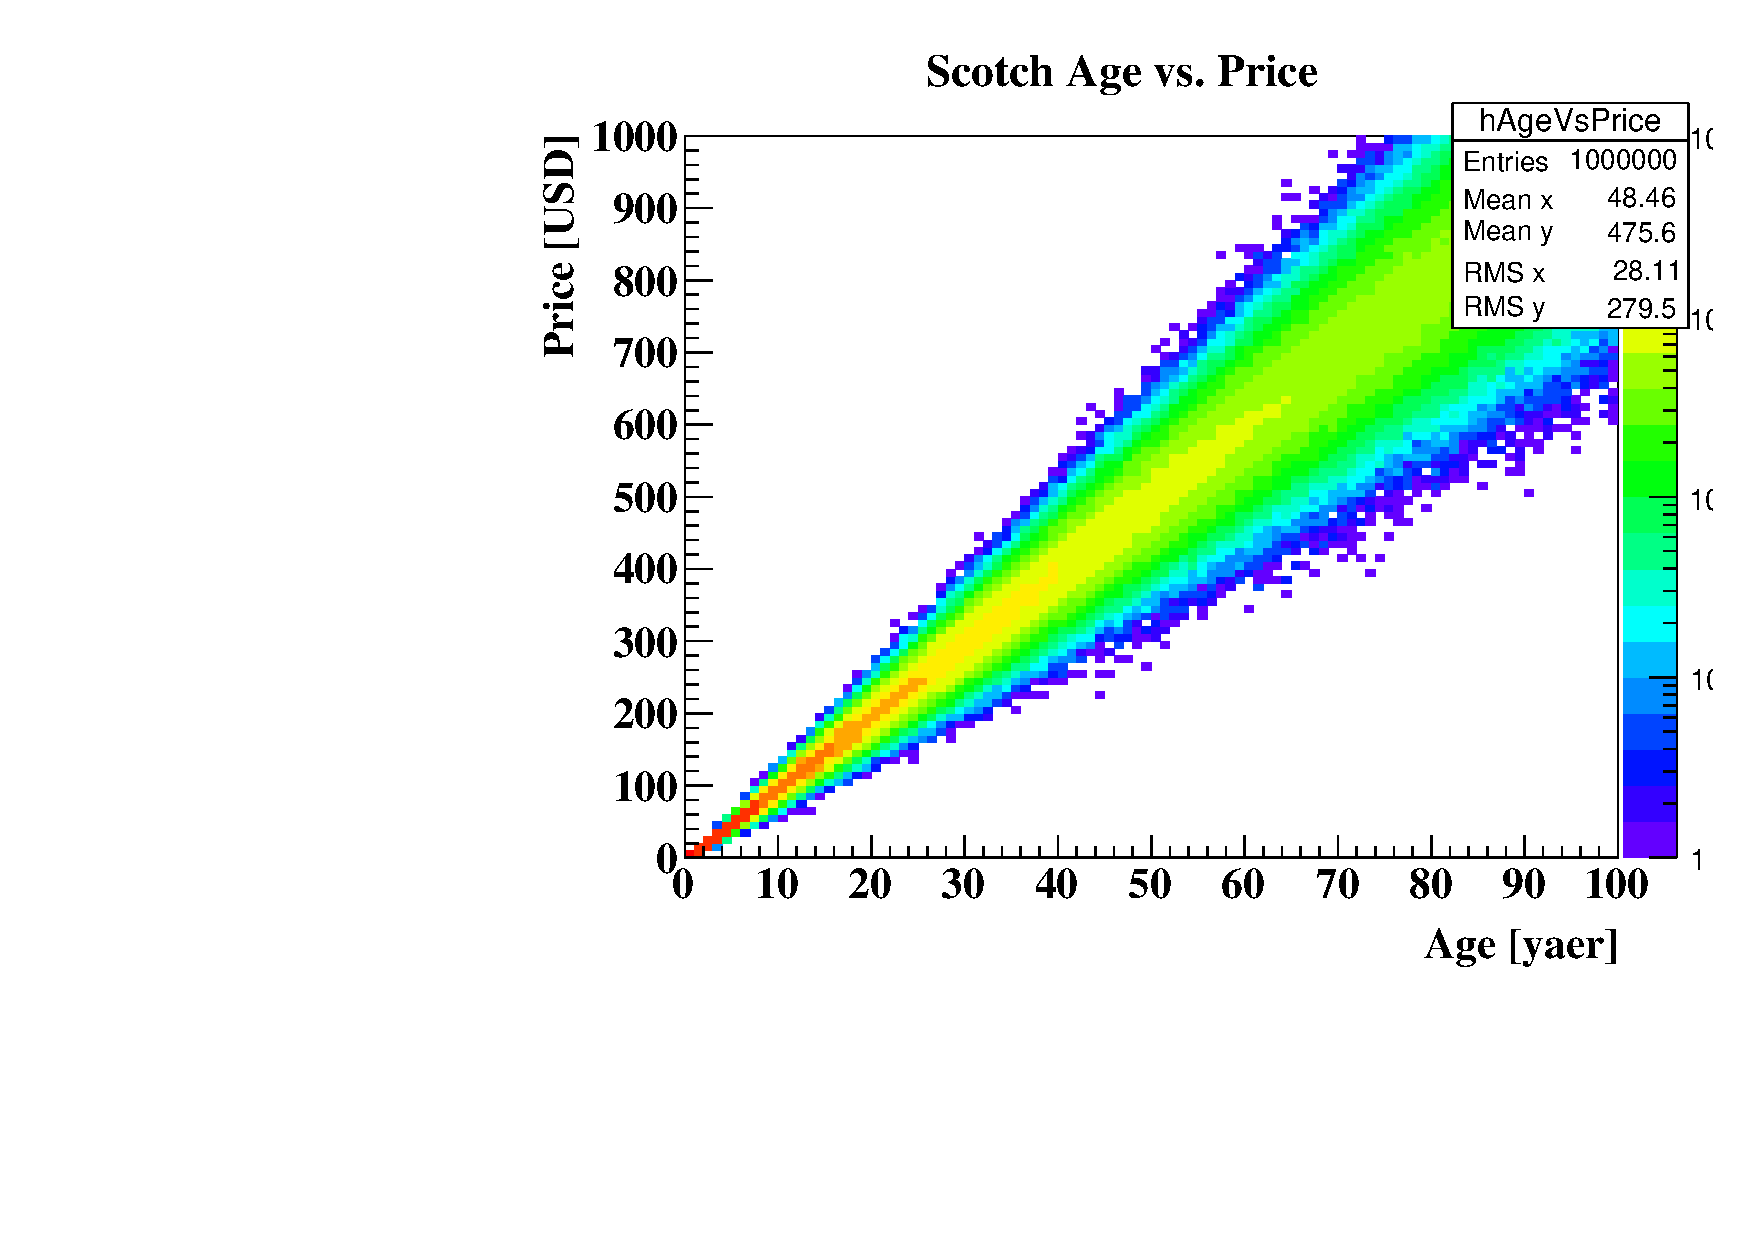
\includegraphics[width=12cm]{./img/ScotchAgeVsPrice.pdf}
\caption{ 
Drawing the age vs. price distribution of {\ttfamily example::Scotch} class from {\ttfamily TTree::Draw}.
}
\end{center}\end{figure}

An example script {\ttfamily mac/example.py} demonstrates how you can:
\begin{itemize}
\item Instantiate {\ttfamily example::Scotch} and save it in a \ROOT file
\item Create a {\ttfamily TTree} of {\ttfamily example::Scotch} for 1e6 entries and save
\item Read-in stored {\ttfamily TTree} and make a very simple access to the stored data product
\item Read-in stored {\ttfamily TTree} and call {\ttfamily TTree::Draw} on the stored data product
\end{itemize}

Note that storing multiple variables into a separate branch of {\ttfamily TTree} (i.e. Ntuple approach)
is much more tedious than storing a class instance as demonstrated in {\ttfamily Scotch::ShipScotch}
function. There, you can find a single line to create a {\ttfamily TTree} branch:
\begin{lstlisting}
tree.Branch("scotch",&data);
\end{lstlisting}
where ``data'' is a {\ttfamily example::Scotch} instance.
With this single line call, all variables in {\ttfamily example::Scotch} instance is stored
with a proper type, and will be readout correctly.

Another myth often people have is that it is very hard to access this object information from
{\ttfamily TTree}. As you can see in the {\ttfamily example.py}, this is completely irrelevant:
you can access the object directly via branch name. A single line in {\ttfamily Python} from
the script is shown below:
\begin{lstlisting}
ch.scotch.Speak()
\end{lstlisting}
which accesses the stored object and calling the class member function {\ttfamily example::Beer::Speak()}.

\subsection{Package Dependency}
The package {\ttfamily Example/Dependent} is prepared to demonstrate how one can make an inter-package 
dependency. In particular, this package depends on {\ttfamily Example/Function} package. Make sure
you have finished building {\ttfamily Example/Function} before building this package.

As you can see in {\ttfamily Stout.h}, the \CPP class {\ttfamily example::Stout} inherits from
{\ttfamily example::Beer}. In order to avoid re-compilation of {\ttfamily example::Beer} class,
we take a usual approach of just {\it linking} the libraries together. Take a look at 
{\ttfamily GNUmakefile}, in particular the following lines:
\begin{lstlisting}
...
INCFLAGS += -I$(LARLITE_USERDEVDIR)/Example
...
LDFLAGS += -L$(LARLITE_LIBDIR) -lExample_Function
\end{lstlisting}
As advertised in the previous section, you must include the path to find {\ttfamily Beer.h} (which
is called from {\ttfamily Stout.h} via {\ttfamily \#include ``Beer.h''}) in {\ttfamily INCFLAGS}, and
both a path and name of a library that contains {\ttfamily example::Beer} class definition in
{\ttfamily LDFLAGS}. 

An example script {\ttfamily mac/example.py} demonstrates an instantiation of {\ttfamily example::Stout}
class and also a call to its base class function {\ttfamily example::Beer::Speak()}.

\subsection{\python in \CPP}
Finally, some users are interested in developing \CPP code to directly operate on \python objects.
An example {\ttfamily Example/PyExample} is prepared to give a tip on how one can write a \CPP
API for \python. This is much better documented as a part of \python documentation:
\begin{center}
{\color{blue}\url{https://docs.python.org/2/c-api/}}
\end{center}

Using a native \python \CPP API is not very easy nor straight forward. Hence in this example,
again, we use \PyROOT binding that makes our life much easier. In short, a difference of two
methods is that you do not have to write your own binding, which is an extra code that has nothing
to do with your algorithm. Finally, that being said, there are other bindings available out there
such as {\ttfamily Cython} (... and \PyROOT uses one of them underneath anyways).

\subsubsection{External Dependnecy}
First of all, you will be using native \python classes, hence you will depend on \python.
Accordingly you have to modify {\ttfamily GNUmakefile}, in particular {\ttfamily INCFLAGS} and
{\ttfamily LDFLAGS}. Notice following 2 lines in {\ttfamily GNUmakefile}:
\begin{lstlisting}
...
INCFLAGS += $(shell python-config --includes)
...
LDFLAGS += $(shell python-config --ldflags)
\end{lstlisting}
each specifying an extra path to find a \python header file and libraries.

\subsubsection{Hiding \python Header From \CINT}
\python header file is called {\ttfamily Python.h}, and is not parse-able via \ROOT \CINT
compiler. So you have to hide it from \CINT dictionary generation step. This can be seen
in {\ttfamily PyExample.h} header file:
\begin{lstlisting}
...
#ifndef __CINT__
// You have to hide native Python header include from CINT                                                                                                                                                  
#include "Python.h"
#endif
...
\end{lstlisting}

You also need to provide two magic lines to forward declare types:
\begin{lstlisting}
...
struct _object;
typedef _object PyObject;
...
\end{lstlisting}
which is for \python generic object pointers to be used (this is a part of \python \CPP API).

\subsubsection{{\ttfamily example::PyExample::Convert}}
The example class {\ttfamily example::PyExample} has an example function to create a
\python list from a \CPP {\ttfamily std::vector<std::string>} object. You can look at the
source code as to how one can do this very simple operation, and take a look at \python
documentation for doing more elaborate operations.

Running {\ttfamily mac/example.py} should show you how this function works.
Obviously you may want to expand the code to work with more advanced \python objects
such as {\ttfamily numpy} array, {\ttfamily matplotlib} axis, and such. The author
does not have much experience to extend too far, but is happy to discuss if you need a help.

\subsection{Documenting Code Using {\ttfamily Doxygen}}
Though this is not everyone's favorite choice, {\ttfamily doxygen} is a popular method to
provide an in-line documentation in the source code. It works pretty nicely with \CPP, and
somewhat at acceptable level with \python. It is the recommended choice for LArSoft to provide
a minimal documentation.

LArLite repositories comes with a doxygen script. You can try generating a documentation
in {\ttfamily Example} directory by typing:
\begin{lstlisting}
  > make doxygen
\end{lstlisting}
({\bf you need doxygen installed in your system!}).

\begin{figure}[htb]\begin{center}
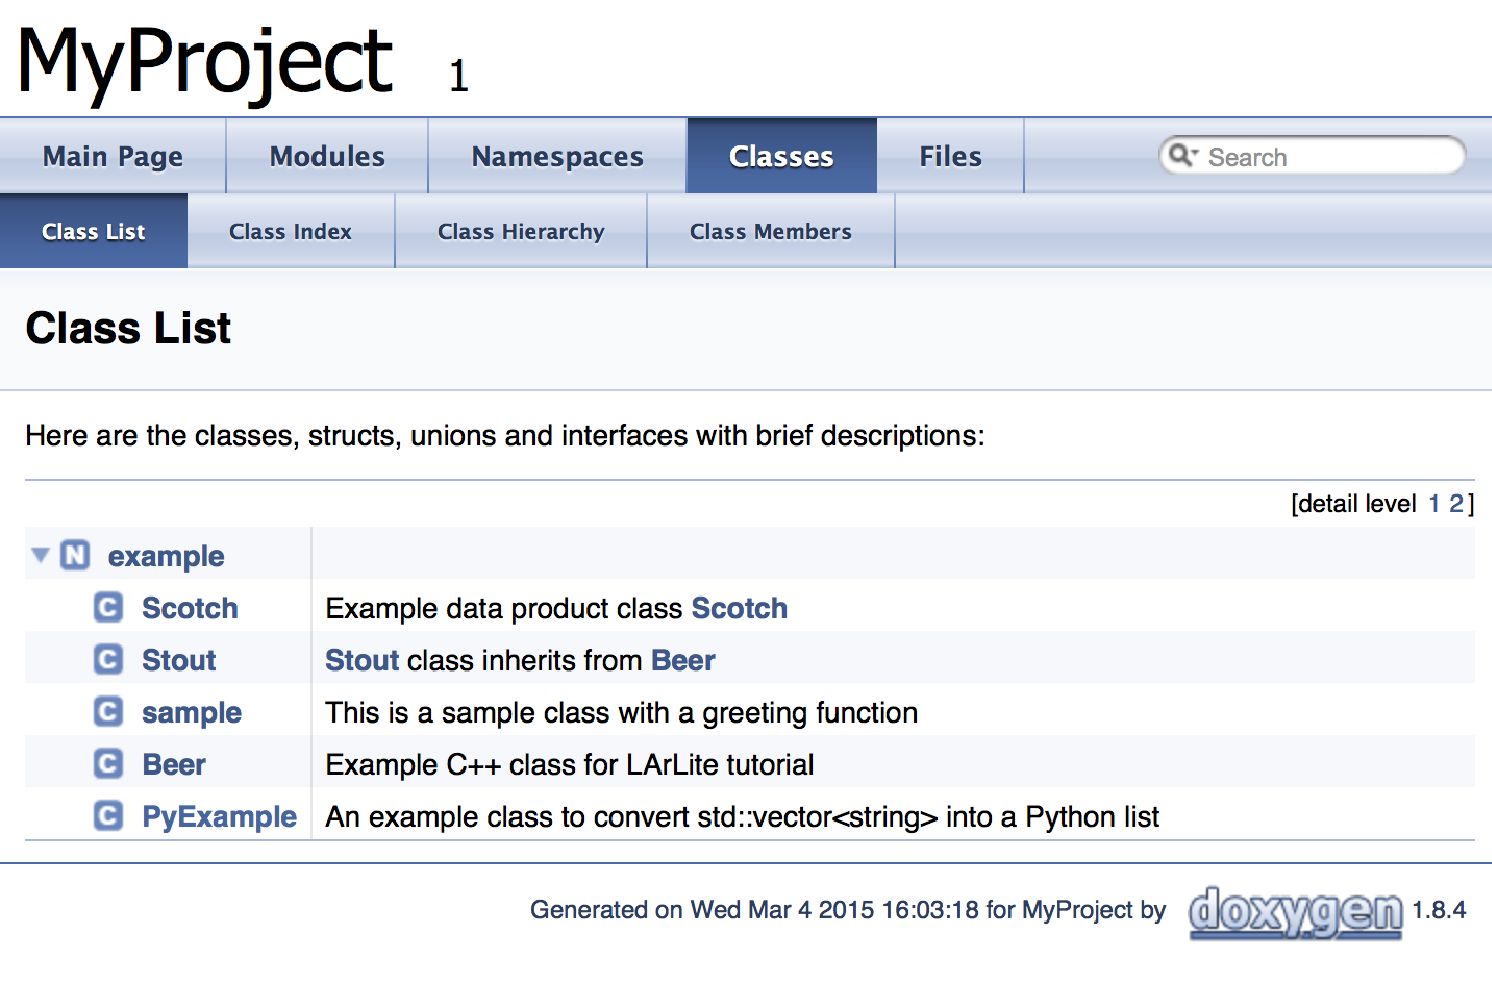
\includegraphics[width=12cm]{./img/doxygen.pdf}
\caption{ 
Doxygen web page generated by ``{\ttfamily make doxygen}'' command for {\ttfamily Example} repository.
}
\end{center}\end{figure}

After successfully running the above command, you should find a chain of HTML files 
to browse through (no internet needed). This way you can also check your doxygen comment
format (whether this is correct or not) before you commit the code. You can look at the
generated documentation using a command like below:
\begin{lstlisting}
  > firefox -a doc/dOxygenMyProject/html/index.html 
\end{lstlisting}
on {\ttfamily Linux} or
\begin{lstlisting}
  > open doc/dOxygenMyProject/html/index.html 
\end{lstlisting}
on {\ttfamily OSX}. The figure shows a generated documentation webpage on the author's laptop.

To understand {\ttfamily doxygen} comment style, refer to their web documentation:
\begin{center}
{\color{blue}\url{http://www.stack.nl/~dimitri/doxygen/manual/docblocks.html}}
\end{center}
